\newpage
IRSTI 61.01.05

\sectionwithauthors{A.I.Samadun, B.R. Taussarova, Zh.S. Nabiyev., G.T.Daribayeva}{DEVELOPMENT OF ANTIMICROBIAL PACKAGING MATERIALS FOR FOOD
PRODUCTS BASED ON COPPER NANOPARTICLES}

\begin{center}
{\bfseries A.I.Samadun, B.R. Taussarova, Zh.S. Nabiyev., G.T.Daribayeva}

Almaty Technological University, Almaty, Kazakhstan

Corresponding author: abdu.93\_93@mail.ru
\end{center}

In the process of storage and delivery, food products are subjected to
physical changes, resulting in moisture exchange between the product and
the environment, mechanical damage, chemical processes occurring in the
product itself, as well as microbiological damage. The use of packaging
materials on the basis of polyolefins, reduce the influencing factors
leading to rapid corruption of food products. However, by their nature,
polyethylene and polypropylene films do not have antimicrobial
properties. Therefore, in order for the packaging based on them to
protect the product from microbiological damage, various technological
techniques are used for the processing of packaging, as well as the
introduction of special antimicrobial agents into the composition of the
film. The present study developed a method of synthesis of copper oxide
nanoparticles stabilized with gelatin and pectin. The synthesis was
carried out by direct chemical sedimentation. Copper chloride was used
as a precursor to the synthesis of copper oxide. Gelatin and pectin were
used as stabilizers. Gelatin and pectin were used as a stabilizer as an
environmentally friendly component of the film. In addition, consumers
are interested in innovative, economical, harmless and effective food
packaging materials.

The results showed that CuO nanoparticles, stabilized with gelatin and
pectin, have a high potential for use in food packaging - both as a
stand-alone nanoplane and as part of other packaging materials.

{\bfseries Key words}: CuO nanoparticles, gelatin, pectin, polylactide,
antimicrobial, packaging.

\sectionheading{МИКРОБҚА ҚАРСЫ ТАҒАМДЫҚ ҚАПТАМА МАТЕРИАЛДАРЫН МЫС
НАНОБӨЛШЕКТЕРІНІҢ НЕГІЗІНДЕ ӘЗІРЛЕУ}

\begin{center}
{\bfseries А.И.Самадун, Б.Р.Таусарова, Ж.С.Набиева, Дарибаева Г.Т.}

Алматы технологиялық университеті, Алматы қ., Қазақстан,

е-mail: abdu.93\_93@mail.ru
\end{center}

Сақтау және сату процесінде тамақ өнімдері физикалық өзгерістерге
ұшырайды, нәтижесінде өнім мен қоршаған орта арасында ылғал алмасу,
механикалық зақымдану, өнімнің өзінде болатын химиялық процестер,
сондай-ақ микробиологиялық бүліну пайда болады. Полиолефиндерге
негізделген орау материалдарын қолдану әсер етуші факторларды азайтуға
мүмкіндік береді, бұл тағамның тез бұзылуына әкеледі. Алайда, табиғаты
бойынша полиэтилен және полипропилен пленкалары микробқа қарсы
қасиеттерге ие емес. Сондықтан, олардың негізінде қаптама өнімді
микробиологиялық бұзылудан қорғау үшін қаптаманы өңдеудің әртүрлі
технологиялық әдістері, сондай-ақ пленкаға, арнайы микробқа қарсы
агенттерге кіріспе қолданылады. Бұл зерттеуде желатин мен пектинмен
тұрақтандырылған мыс оксидінің нанобөлшектерін синтездеу әдісі жасалды.
Синтез тікелей химиялық тұндыру арқылы жүзеге асырылды. Мыс оксидін
синтездеу үшін прекурсорлар ретінде мыс хлориді қолданылды.
Тұрақтандырғыш ретінде желатин мен пектин қолданылды. Желатин мен пектин
экологиялық тұрақтандырғыш өнім ретінде қолданылды. Сонымен қатар,
тұтынушылар инновациялық, үнемді, экологиялық таза және тиімді
азық-түлік қаптама материалдарына қызығушылық танытуда.

Нәтижелер желатин мен пектинмен тұрақтандырылған CuO нанобөлшектерінің
азық - түлік қаптамасында-тәуелсіз нанопленка ретінде де, басқа орау
материалдарының бөлігі ретінде де пайдалану мүмкіндігі жоғары екенін
көрсетті.

{\bfseries Түйін сөздер:} CuO нанобөлшектері, желатин, пектин, полилактид,
микробқа қарсы, орау.

\sectionheading{РАЗРАБОТКА АНТИМИКРОБНЫХ УПАКОВОЧНЫХ МАТЕРИАЛОВ ДЛЯ ПИЩЕВЫХ ПРОДУКТОВ НА ОСНОВЕ НАНОЧАСТИЦ МЕДИ}

\begin{center}
{\bfseries А.И.Самадун, Б.Р.Таусарова, Ж.С.Набиева, Г.Т.Дарибаева}

Алматинский технологический университет, г. Алматы, Казахстан,

е-mail: abdu.93\_93@mail.ru
\end{center}

В процессе хранения и реализации пищевые продукты, подвергаются
физическим изменениям, в результате которых происходит влагообмен между
продуктом и окружающей средой, механическим повреждениям, химическим
процессам, протекающим в самом продукте, а также микробиологической
порче. Применение упаковочных материалов на основе полиолефинов,
позволяют снизить воздействующие факторы, приводящие к быстрой порче
пищевых продуктов. Однако по своей природе полиэтиленовые и
полипропиленовые пленки не обладают антимикробными свойствами. Поэтому
для того, чтобы упаковка на их основе защищала продукт от
микробиологической порчи, применяются различные технологические приемы
по обработки упаковки, а также введение в состав пленки, специальных
антимикробных агентов. В настоящем исследовании был разработан метод
синтеза наночастиц оксида меди, стабилизированных желатином и пектином.
Синтез осуществлялся путем прямого химического осаждения. В качестве
предшественников для синтеза оксида меди использовались хлорид меди. В
качестве стабилизатора использовался желатин и пектин. Как экологически
продукт в качестве стабилизатора использовался желатин и пектин. Кроме
того, потребители заинтересованы в инновационных, экономичных,
экологически чистых и эффективных упаковочных материалах для пищевых
продуктов.

Результаты показали, что наночастицы CuO, стабилизированные желатином и
пектином, обладают высоким потенциалом для использования в упаковке
пищевых продуктов - как в качестве самостоятельной нанопленки, так и в
составе других упаковочных материалов.

{\bfseries Ключевые слова:} наночастицы CuO, желатин, пектин, полилактид,
антимикробная, упаковка.

\begin{multicols}{2}
{\bfseries Introduction.} The issue of healthy and high-quality nutrition
is global. In developing countries, this problem is linked to
underdeveloped agriculture and processing.

The high rate of urbanization has forced the population of large cities
to switch to industrial methods of food supply. Such methods require
various measures aimed at significantly extending the shelf life of
food. This constantly leads to a decrease in the nutritional value of
foodstuffs. As the population continues to grow, these challenges will
have an increasing impact on the global food distribution system,
creating imbalances between regions with varying levels of economic
development.

There are various ways to address the above challenges: agricultural
development, improved food supply chains, sustainable production and
consumption. An important factor in ensuring food security is the
development of methods to increase the shelf life of food products
without significantly reducing their quality. Such methods for extending
shelf life include the use of antimicrobial packaging. Antimicrobial
packaging is made by modifying traditional packaging to provide
protection against the growth of pathogens during food storage.

Nanoparticles are often used in the food industry to create
antibacterial films {[}1, 2{]}. Research is currently under way to
develop antimicrobial packaging materials derived from various
nanoparticles, including CuO {[}3-5{]}. Nanopackets can be applied to
food products by wrapping, grinding, brushing or spraying to provide a
selective barrier against the movement of gases, moisture and dissolved
materials, as well as protection against mechanical damage {[}6, 7{]}.
The main development is aimed at obtaining nanoparticles with subsequent
surface treatment of finished packaging materials. According to Kamran
Tahir, Dipranjan Laha, Arindam Pramanik, the activity of nanoparticles
depends on the shape and their dispersion. The stabilization of
nanoparticles is an important aspect in the design of food packaging
with nanocomposites.The bactericidal activity and migration of
nanoparticles into the product depends on the method of synthesis
{[}8{]} and determines the stability of nanoparticles in the polymer
composition of packaging materials. With high stability, migration of
CuO nanoparticles into the product will be eliminated, which guarantees
no toxicity of the packaging material. The safety of food products
during their long-term storage is influenced by a wide range of factors:
adverse influence of the external environment, processes of natural
corruption due to natural biochemical and chemical reactions,
development of microorganisms. Microbiological damage is one of the most
significant factors affecting the preservation of the quality of
foodstuffs, both of plant and animal origin.

Microbiological stability can be achieved in various ways: by adding
preservatives to the product, using special storage technologies, use of
special packaging, etc. Often many methods of preventing microbiological
damage are associated with the influence on the biochemical processes of
the life of living organisms. Along with the effects on microorganisms,
these methods can have a significant effect on a person whose body
functions according to similar biochemical patterns. Thus, the use of
preservatives reduces the quality of the product, use of special
technologies can also lead to a significant loss of nutritional value
and significantly increase the cost of products. One of the most
promising directions to increase the shelf life of foodstuffs is the use
of special packaging materials that can protect the product from
negative environmental factors, as well as reduce the rate of
microbiological damage.

The aim of this work is to development of a method for the synthesis of
CuO nanoparticles stabilised with gelatin and pectin, to study the
possibility of their using in food packaging to protect against
microbiological spoilage and increase the storage life.

{\bfseries Materials and methods.} \emph{CuO Nanoparticles Synthesis
Method.}

Reagents: Copper (II) 2-water chloride (Sigma-Aldrich Pty Ltd, Merck
KGaA branch, Darmstadt, Germany), gelatin (Segma-Aldrich Ptys Ltd, merck
KGAA subsidiary, DARMSTAD, Germany); sodium hydroxide (Shandong Zhoushun
International Trade Co., Ltd); ascorbic acid-L (SIGMA-ALDRICH PTY Ltd,
MERCK KGA A branch, darmstad, Germany) and pectin (Jiaxing Renze Import
\& Export Co., Ltd.).

CuO nanoparticles, stabilized with gelatin and pectin, were polluted by
direct chemical sedimentation. Copper chloride was used as a precursor
to CuO nanoparticles (II). Pectin and gelatin acted as a stabilizer, as
a restorative used ascorbic acid, sodium hydroxide - as a sediment.
Distilled water was used as a reaction medium.

CuO nanoparticles stabilized with gelatin and pectin were obtained by
the following procedure: 0.03 g of precursor (copper chloride), 0.03 g
of gelatine and 0.1 g of ascarbic acid, dissolved in 90 ml of reaction
medium (distilled water), a similar procedure was performed with
pectine. The resulting solution was heated to boil with constant mixing
and an additional 0.5\% solution of NaOH was added to pH-10. The sample
was mixed for 2-3 minutes, cooled to room temperature, mixed at room
temperature for 20 minutes. As a result, copper oxide nanoparticles were
produced. The phase of obtaining nanoparticles is an important component
of the work on the creation of nanocomposite packaging materials,
because it is the nanoparticle that gives the newly obtained packaging
unique properties.

For the preparation of packaging material modified by CuO nanoparticles,
polylactic film was used, which is often used in the production of
eco-packages. As a test sample, ordinary polylactic film from ECO
Prodacts Group (Astana) was taken.

As part of the development of nanoparticles preparations - visual
evaluation, microphotography of samples of CuO nanoparticles and data on
the elemental composition were obtained with the scanning electron
microscope INTEGRA TERMA and integration of probe and optical microscopy
and spectroscopy, ASM - Raman - SBOM - TERS {[}9{]}. The samples were
dried for study. The samples were prepared as follows: a two-sided
conductive carbon tape was glued to the standard toolboard. CuO powder
was applied to the conductive carbon tape. They then applied a carbon
coating about 10 nm thick. The pH was measured using the Testo 206 ph1
pH meter using a silver chloride combined electrode.

Microbiological analysis methods were used to study the antimicrobial
effectiveness of polylactide films modified with CuO nanoparticles on
bread shelf life.

The effects of polylactid films modified by CuO nanoparticles on the
quality and shelf life of bread were studied.

For the experiment they took white wheat bread produced by "Aksai nan"
(Almaty). The shelf life at the time of purchase was 3 days. In order to
study the initial parameters of the bread on the day of beginning of the
experiment, slices weighing 50±0.2g corresponding to the number of
experimental films were cut.

The bread samples were stored in the SCTC TS-1/80 SPU thermostat at 25 ±
1°C for 120 ± 3 hours of the experiment. After the time passed,
microbiological analysis was carried out. The analysis was carried out
according to GOST 10444.12-2013 Microbiology of food and animal feed.
Methods of detection and counting of yeast and mold mushrooms {[}10{]}.

{\bfseries Results and discussion.} The color of nanoparticles is an
important qualitative characteristic, because it can characterize the
size of particles and their chemical composition. The reason for the
difference in colour of colloid nanoparticles solutions is different:
the nature of the dispersion phase and the disspersion medium, particle
dispersiveness, shape and structure. All these factors affect not only
the absorption of light in the solution, but also its dispersion. Even a
slight change in the color of the solution may indicate a change in
particle size and chemical composition. Figure - 1 shows solutions of
silver nanoparticles obtained by different methods and having different
sizes.
\end{multicols}

\begin{figure}[H]
	\centering
	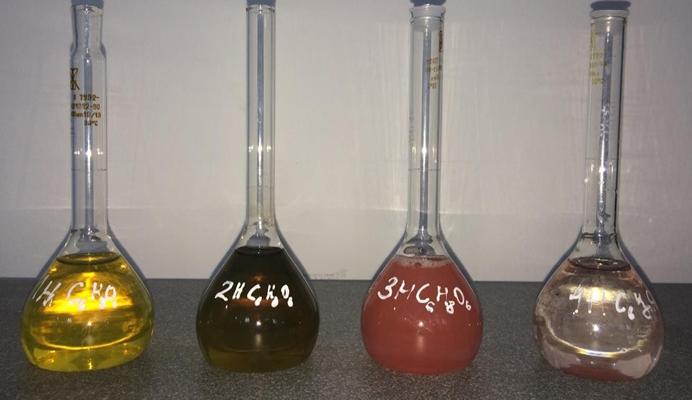
\includegraphics[width=0.8\textwidth]{assets/14}
	\caption*{Fig. 1 - Appearance of copper nanoparticles solutions}
\end{figure}

\begin{multicols}{2}
The optical spectrum of nanoparticles and nanomaterials solutions is no
less important qualitative characteristic than the color of the
solution. The method of optical spectroscopy is based on the measurement
of particle absorption of the electromagnetic radiation of the optical
range. Figure 2, 3, 4 shows the optical spectra for the colloidal
solutions studied.
\end{multicols}

\begin{figure}[H]
	\centering
	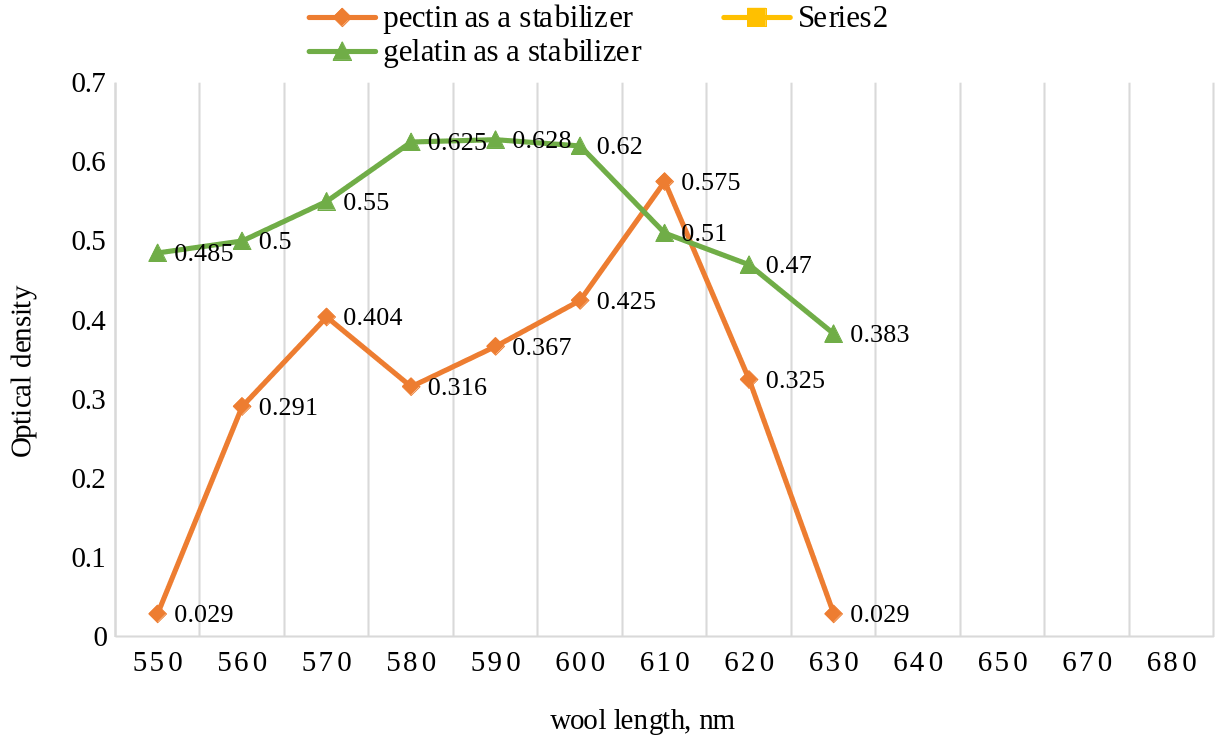
\includegraphics[width=\textwidth]{assets/14.1}
	\caption*{Fig. 2 - Graph of obtained data on spectroscopic photometer Jenway 6705}
\end{figure}

\begin{figure}[H]
	\centering
	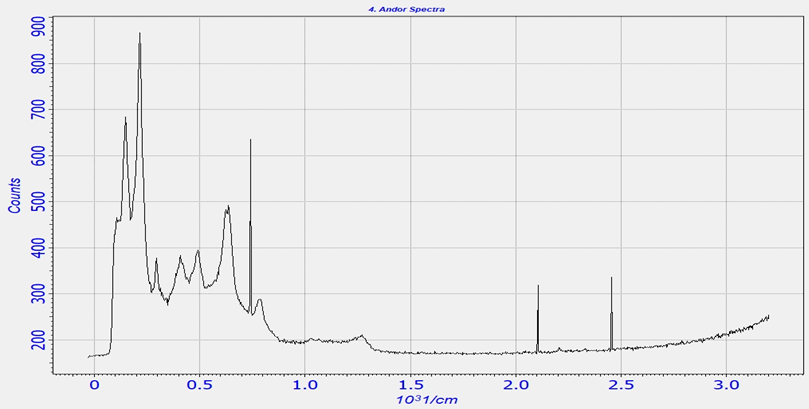
\includegraphics[width=\textwidth]{assets/15}
	\caption*{Fig. 3 - Optical spectrum of copper nanoparticles using gelatin as a stabilizer in exhaust solutions}
\end{figure}

\begin{figure}[H]
	\centering
	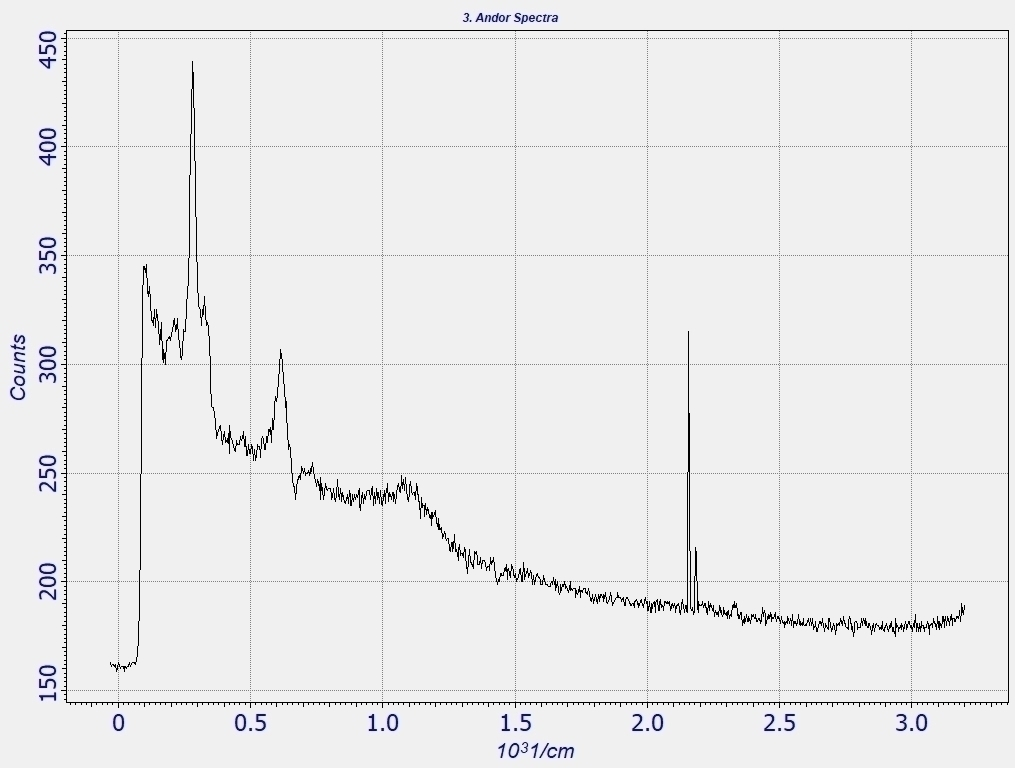
\includegraphics[width=0.8\textwidth]{assets/16}
	\caption*{Fig. 4 - Optical spectrum of copper nanoparticles when pectin is used as a stabilizer in baseline solutions}
\end{figure}

\begin{figure}[H]
    \centering
    \begin{subfigure}[b]{0.45\textwidth}
        \centering
        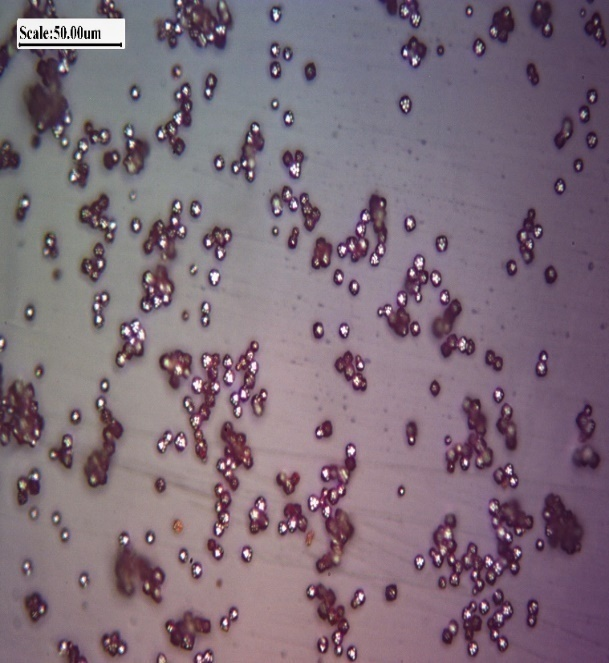
\includegraphics[width=\textwidth]{assets/17}
    \end{subfigure}
    \hfill
    \begin{subfigure}[b]{0.45\textwidth}
        \centering
        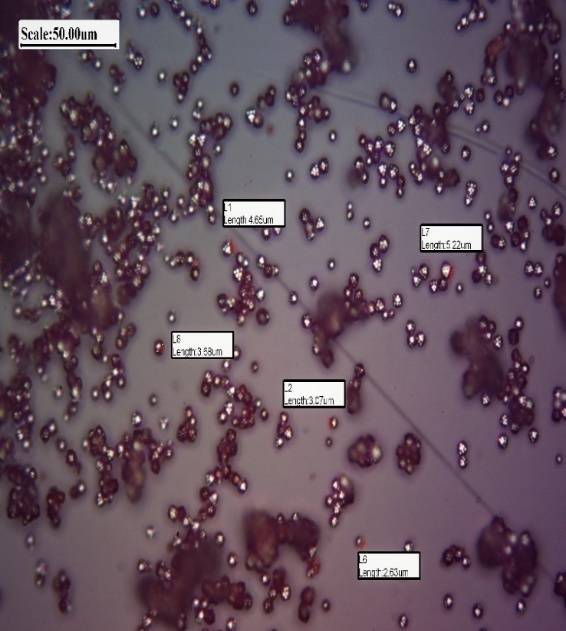
\includegraphics[width=\textwidth]{assets/18}
    \end{subfigure}
    \caption*{Fig. 5 - Optical imaging of copper nanoparticles in the 50 μm range}
\end{figure}

\begin{multicols}{2}
Dispersion phase particle size is one of the most important
characteristics of colloidal solutions, determining their many
properties. In particular, the stability of the solution and its
biological properties may depend on the size of the nanoparticles
{[}11{]}. The samples showed nanoparticles with sizes ranging from 136
to 995 nm. When pectin was used as a stabiliser, and when gelatin was
used as a stabiliser, the particle sizes ranged from 62 to 313 nm.
Photos of samples made by optical and scanning electron microscope are
shown in Figures 5 - 7. Based on the results of scanning and
transmission microscopy, nanoparticles as seen in Figure 7 have
spherical shape like granules. Figure - 8 shows the surfaces of the
films before and after treatment with copper nanoparticles. In the
treated film the clusters of nanoparticles reached up to 500 nm in some
places.
\end{multicols}

\begin{figure}[H]
    \centering
    \begin{subfigure}[b]{0.45\textwidth}
        \centering
        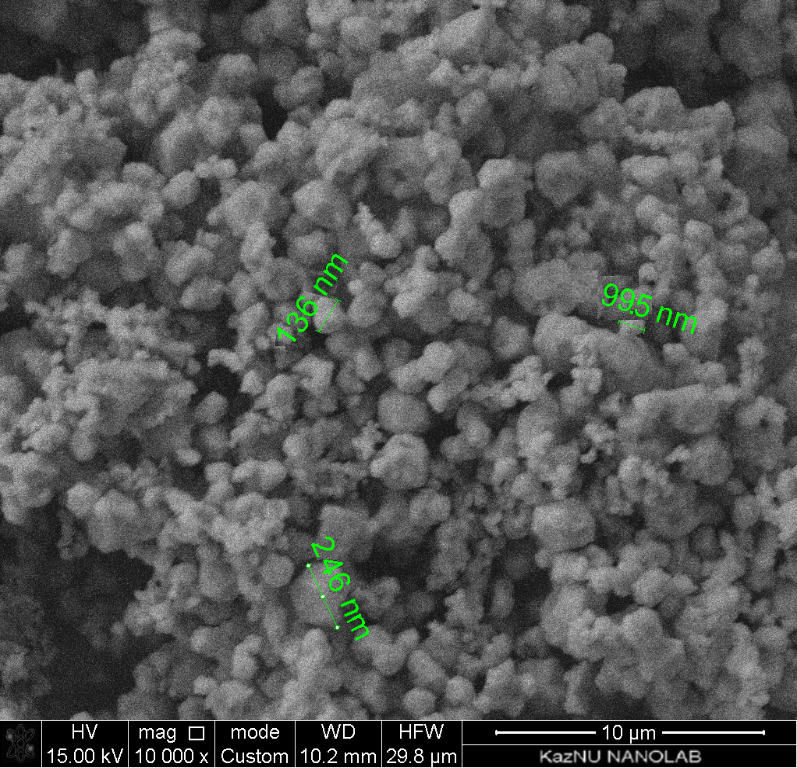
\includegraphics[width=\textwidth]{assets/19}
        \caption*{Fig. 6 - Dimensions of copper nanoparticles using pectin as a stabilizer}
    \end{subfigure}
    \hfill
    \begin{subfigure}[b]{0.45\textwidth}
        \centering
        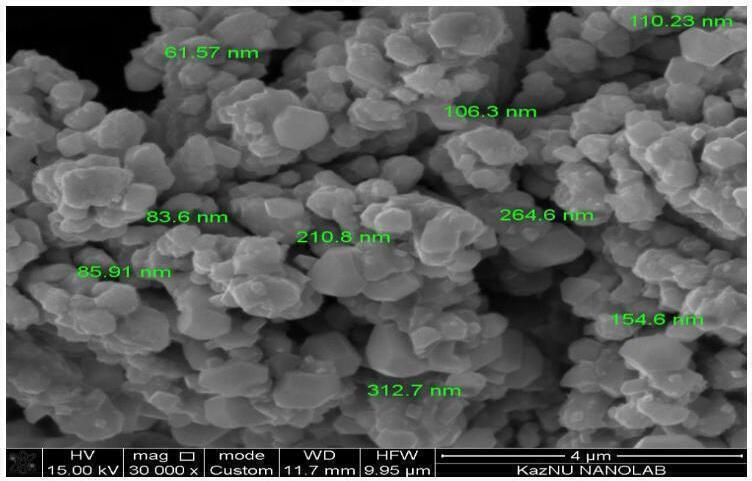
\includegraphics[width=\textwidth]{assets/20}
        \caption*{Fig. 7 - Dimensions of copper nanoparticles using gelatin as a stabilizer}
    \end{subfigure}
\end{figure}

\begin{figure}[H]
    \centering
    \begin{subfigure}[b]{0.45\textwidth}
        \centering
        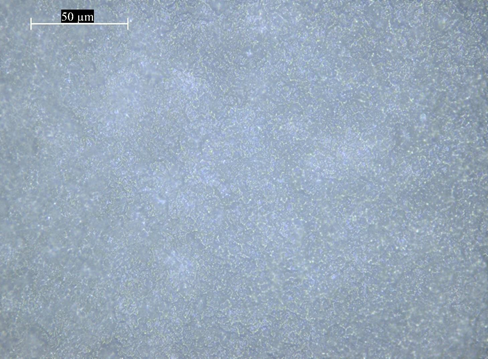
\includegraphics[width=\textwidth]{assets/21}
        \caption*{a}
    \end{subfigure}
    \hfill
    \begin{subfigure}[b]{0.45\textwidth}
        \centering
        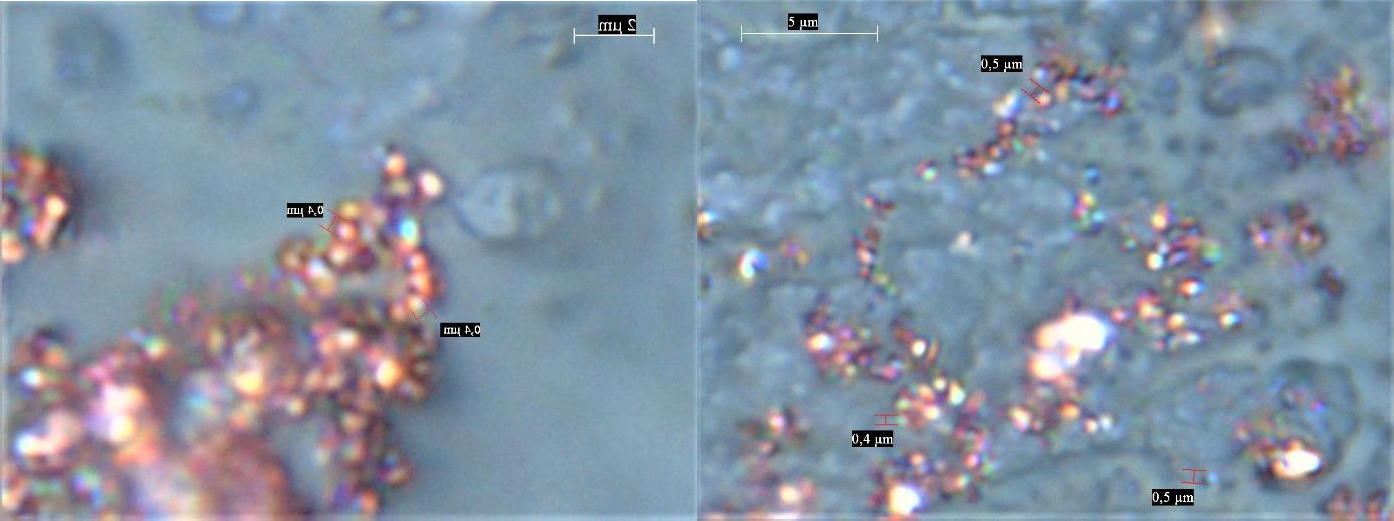
\includegraphics[width=\textwidth]{assets/22}
        \caption*{b}
    \end{subfigure}
    \caption*{Fig. 8 - Polylactid film samples (a) before treatment and (b) after copper nanoparticles treatment}
\end{figure}

\begin{multicols}{2}
As a result of the study of the basic physico-chemical characteristics
of nanoparticle solutions, it can be concluded that they differ strongly
and as a consequence different effects when they are used to create
composite packaging materials. Evaluation of the effectiveness of the
application of a product is an important part of its development
process. Since often not individual characteristics of a product are the
reason for its purchase, but the ability of the product to solve a
particular problem, it is important to determine the possibility of
solving the problem. For nanopackaging, this problem is the extension of
the shelf life of the products packaged in it. The benefits of use can
be significant if such packaging is used as effectively as possible.

In order for the packaging to be used effectively, it is necessary to
determine an extended shelf life compared to conventional packaging. It
is known that the main cause of damage is the development of various
microorganisms, so the use of packaging with antimicrobial agents is
relevant. The shelf life can be determined in different ways, depending
on the type of product.

The method of microbiological testing is most appropriate if the cause
of damage is mainly the development of microorganisms in the product. In
this case, both the total number of microorganisms (COE) can be measured
and differentiated depending on the type of micro-organism. The
advantage of this method is the ability to identify the main source
causing the damage of the product.

The effects of CuO-modified polylactid films on changes in the
microbiological purity of bread storage are further studied in Table 1
and Figure 9.
\end{multicols}

\begin{table}[H]
\caption*{Table 1 - Dynamics of changes in microbiological parameters of bread samples during storage}
\centering
\begin{tabular}{|l|p{0.3\textwidth}|lllllll|}
\hline
\multirow{2}{*}{№} & \multirow{2}{*}{Sample} & \multicolumn{7}{l|}{Mold 			index, CFU/g} \\ \cline{3-9} 
 &  & \multicolumn{1}{l|}{1 			day} & \multicolumn{1}{l|}{2 			day} & \multicolumn{1}{l|}{3 			day} & \multicolumn{1}{l|}{4 			day} & \multicolumn{1}{l|}{5 			day} & \multicolumn{1}{l|}{6 			day} & 7 			day \\ \hline
1 & Bread 			without packaging & \multicolumn{1}{l|}{-} & \multicolumn{1}{l|}{-} & \multicolumn{1}{l|}{1} & \multicolumn{1}{l|}{3} & \multicolumn{1}{l|}{5} & \multicolumn{1}{l|}{8} & 17 \\ \hline
2 & Bread 			with a control package without processing & \multicolumn{1}{l|}{-} & \multicolumn{1}{l|}{-} & \multicolumn{1}{l|}{1} & \multicolumn{1}{l|}{2} & \multicolumn{1}{l|}{3} & \multicolumn{1}{l|}{4} & 10 \\ \hline
3 & Bread 			with processed packaging (using gelatin as a stabilizer) & \multicolumn{1}{l|}{-} & \multicolumn{1}{l|}{-} & \multicolumn{1}{l|}{-} & \multicolumn{1}{l|}{-} & \multicolumn{1}{l|}{1} & \multicolumn{1}{l|}{2} & 4 \\ \hline
4 & Bread 			with processed packaging (using pectin as a stabilizer) & \multicolumn{1}{l|}{-} & \multicolumn{1}{l|}{-} & \multicolumn{1}{l|}{-} & \multicolumn{1}{l|}{-} & \multicolumn{1}{l|}{1} & \multicolumn{1}{l|}{2} & 5 \\ \hline
\end{tabular}
\end{table}

\begin{multicols}{2}
In accordance with the results presented in Table 1 and Figure 9, films
modified with CuO nanoparticles were found to reduce mold growth and
development in experimental bread samples compared to the control bread
sample. The data obtained shows the activity of CuO nanoparticles
stabilized with gelatin and pectin, and also coincides with the data of
other authors {[}12, 13{]}, who studied the antibacterial activity of
CuO nanoparticles.
\end{multicols}

\begin{figure}[H]
	\centering
	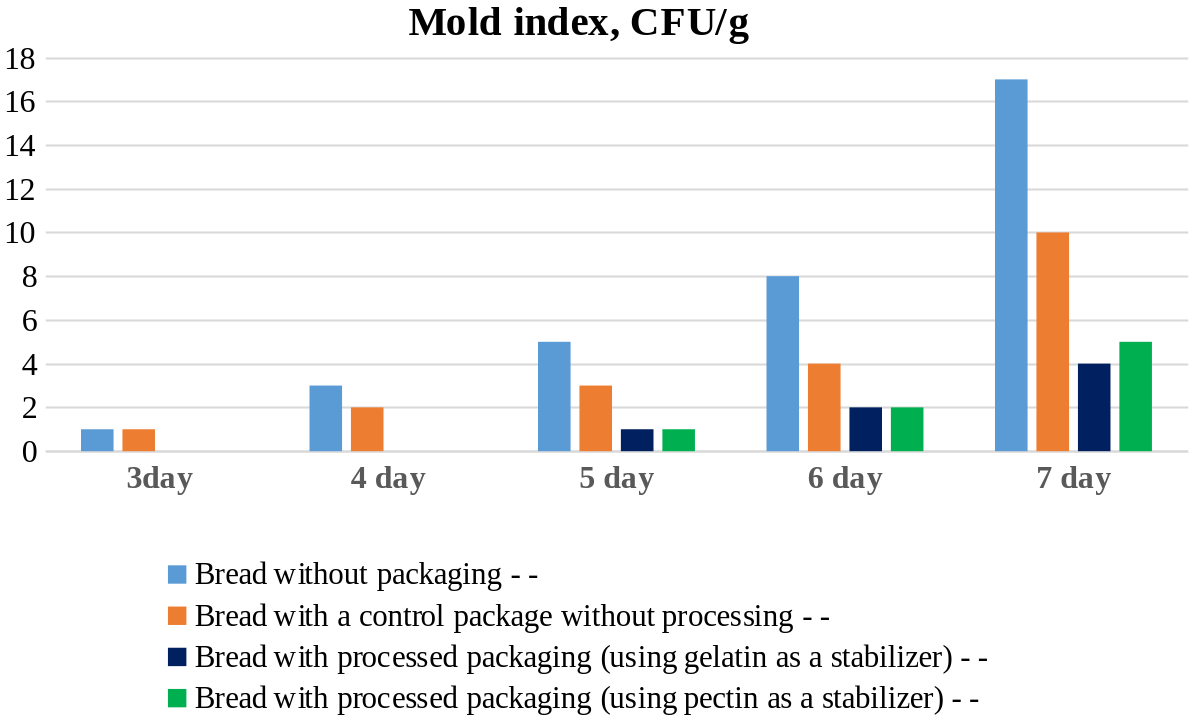
\includegraphics[width=0.9\textwidth]{assets/22.1}
	\caption*{Fig. 9 - Effect of polylactide packages treated with copper nanoparticles on microbiological parameters}
\end{figure}

\begin{multicols}{2}
{\bfseries Conclusions.} The problem of healthy and quality nutrition,
along with the problem of adequacy of such nutrition is relevant for
modern humanity. One way of addressing this problem, as discussed in
this paper, is to keep products fresh and suitable for consumption for a
considerable period of time. Fortunately, modern technologies allow to
obtain and explore the latest materials that can be used to solve the
above-mentioned problems. As a result of the studies carried out and
presented in this paper, the following conclusions can be drawn:

1. A method of synthesis of CuO nanoparticles stabilized with gelatin
and pectin has been developed, their colloidal stability in various
dispersion media has been studied and their possibility of use in bread
packaging has been explored.

2. The results showed that the use of copper chloride as a precursor
allows to produce copper oxide (II). According to the data, copper oxide
nanoparticles stabilized by gelatin and pectin in the aquatic
environment had particles of the smallest diameter of 62 nm.

3. It has been found that CuO nanoparticles, stabilized with gelatin and
pectin, have antimicrobial activity and can be used as a material for
food nanopackets, providing an increase in the shelf life of products,
as shown in the example of bread. The high level of stability of CuO
nanoparticles stabilized with gelatin and pectin will also facilitate
their use in the creation of active food packaging materials.

4. It was found that polylactic films modified by CuO nanoparticles
inhibited mold growth and development in experimental bread samples.

5. The morphology of the surface is studied by electronic microscopy.
The result showed that when using gelatin as a stabilizer, the maximum
copper nanoparticles size was 313 nm, and when using pectin, the
particle size was 246 nm.

Thus, the results of experiments show that CuO nanoparticles, stabilized
with gelatin and pectin, have a high potential for use in food packaging
- both as a self-propelled nanofilm and as part of other packaging
materials, and can also be laid as a basis for food interaction studies,
the environment and be useful for developers engaged in the creation of
promising packaging material.
\end{multicols}

\begin{center}
{\bfseries References}
\end{center}

\begin{noparindent}
1. Osovskaya I.I., Baranova A.E. Rastvory agara dlja uluchshenija
kachestva upakovochnyh bumazhnyh materialov,
tekstil\textquotesingle nyh i kozhanyh izdelij. // Tehnologija
tekstil\textquotesingle\textquotesingle noj promyshlennosti, №5 (407)
2023, pp 129-132. DOI 10.47367/0021-3497\_2023\_5\_129.

2. Baranchikov A.E. Sonohimicheskij sintez neorganicheskih materialov./
A.E. Baranchikov, V.K. Ivanov, Ju.D. Tret\textquotesingle jakov.//
Uspehi himii, 76, 147 (2007).

3. Galiahmetov R.N. Poluchenie nanochastic Cu2O v uslovijah
ul\textquotesingle trazvukovoj kavitacii./ R.N. Galiahmetov, A.G.
Mustafin, R.R. Garafutdinov, G.M. Kuznecova.// Pis\textquotesingle ma
o materialah T.1. 2011. str 176-178.

4. Abdullah, A.S., Essa, F.A., Bacha, H.B. \& Omara, Z.M. Improving the
trays solar still performance using reflectors and phase change
material with nanoparticles // J Energy Storage 31, 101744. 2020. DOI

10.1016/j.est.2020.101744

5. Magonov, S., Belikov, S., Surtchev, M., Leesment S., Malovichko I.
High-Resolution Mapping of Quantitative Elastic Modulus of Polymers //
Microscopy and Microanalysis. 2015. Vol. 21 (S. 3). P. 2183-2184. DOI

10.1017/S1431927615011691.

1. GOST 10444.12-2013 Mikrobiologiya pishchevykh produktov i kormov dlya
zhivotnykh. Metody vyyavleniya i podscheta kolichestva drozhzhey i
plesnevykh gribov. - Moskva: Standartinform, 2014. - 9 s. {[}in
Russian{]}

6. Gvozdenko, A.A., Siddiqui, S.A., Blinov, A.V. et al. Synthesis of CuO
nanoparticles stabilized with gelatin for potential use in food
packaging applications // Sci Rep. 2022. Vol 12. DOI
10.1038/s41598-022-16878-w.

7. Singh, P.K., Das, A.K., Hatui, G. \& Nayak, G.C. Shape controlled
green synthesis of CuO nanoparticles through ultrasonic assisted
electrochemical discharge process and its application for
supercapacitor // Mater. Chem. Phys. -2017. -P. 16-34 DOI:
10.1016/j.matchemphys.2017.04.070.

8. Jana, R. et al. Improving performance of device made up of CuO
nanoparticles synthesized by hydrothermal over the reflux method //
Applied Surface Science. 2018. Vol. 452. P. 155-164.
DOI:10.1016/j.apsusc.2018.04.262.

9. Pelegrino, M.T. et al. Effects of copper oxide nanoparticles on growth
of lettuce (Lactuca sativa L) seedlings and possible implications of
nitric oxide in their antioxidative defense // Environ. Monit. Assess.
2020. Vol. 192. -P. 232-246. DOI: 10.1007/s10661-020-8188-3.

10. Pestovsky, Y. S. \& Martínez-Antonio, A. The use of nanoparticles and
nanoformulations in agriculture // J. Nanosci. Nanotechnol. -2017.
Vol. 17. P. 8699-8730 DOI: 10.1166/jnn.2017.15041.

11. Mousa, A. M. et al. Biosynthetic new composite material containing CuO
nanoparticles produced by Aspergillus terreus for 47Sc separation of
cancer theranostics application from irradiated Ca target // Appl.
Radiat. Isot. 2020. Vol. 166, DOI: 10.1016/j.apradiso.2020.109389.

12. Abdullah, A. S., Essa, F. A., Bacha, H. B. \& Omara, Z. M. Improving
the trays solar still performance using reflectors and phase change
material with nanoparticles // Journal Energy Storage. 2020. Vol. 31.
DOI: 10.1016/j.est.2020.101744.
\end{noparindent}

\emph{{\bfseries Information about the authors}}

\begin{noparindent}
Samadun A.I. - PhD student, Department of Chemistry, Chemical Technology
and Ecology, Almaty University of Technology,Almaty, Kazakhstan, е-mail:
abdu.93\_93@ mail.ru;

Taussarova B.R. - Professor of the Department of Chemistry, Chemical
Technology and Ecology, D.H.N., Almaty University of Technology, Almaty,
Kazakhstan, е-mail: birtausarova@mail.ru;

Nabiyeva Zh. S. - Director of the Scientific Research Institute of Food
Safety, PhD, Almaty University of Technology, Almaty, Kazakhstan,
е-mail: atu\_nabiyeva@mail.ru;

Daribayeva G.T. - Head of the Food Safety Test Laboratory, PhD, Almaty
University of Technology, Almaty, Kazakhstan, е-mail:
daribaeva.80@mail.ru
\end{noparindent}

\emph{{\bfseries Сведение об авторах}}

\begin{noparindent}
Самадун А.И- докторант кафедры «Химии, химической технологии и экологии»
Алматинский технологический университет, Алматы, Казахстан, е-mail:
abdu.93\_93@ mail.ru;

Таусарова Б.Р.-профессор кафедры «Химия, химическая технология и
экология», д.х.н., Алматинский технологический университет, Алматы,
Казахстан, е-mail: birtausarova@mail.ru;

Набиева Ж.С. - Директор Научно-исследовательского института пищевой
безопасности, доктор PhD, Алматинский технологический университет,
Алматы, Казахстан,

е-mail: atu\_nabiyeva@mail.ru;

Дарибаева Г.Т.- заведующая испытательной лабораторией «Пищевая
безопасность», доктор PhD, Алматинский технологический университет,
Алматы, Казахстан,

е-mail: daribaeva.80@mail.ru
\end{noparindent}
